\documentclass[11pt]{beamer}

\usepackage[utf8]{inputenc}  
\usepackage{polski}
\usepackage{hyperref}

\usetheme{Warsaw}

\newcommand{\backupbegin}{
   \newcounter{finalframe}
   \setcounter{finalframe}{\value{framenumber}}
}
\newcommand{\backupend}{
   \setcounter{framenumber}{\value{finalframe}}
}

\newcommand{\zerodisplayskips}{%
  \setlength{\abovedisplayskip}{0pt}%
  \setlength{\belowdisplayskip}{0pt}%
  \setlength{\abovedisplayshortskip}{0pt}%
  \setlength{\belowdisplayshortskip}{0pt}}
\appto{\normalsize}{\zerodisplayskips}
\appto{\small}{\zerodisplayskips}
\appto{\footnotesize}{\zerodisplayskips}

\DeclareMathOperator*{\argmax}{arg\,max}
\newtheorem{lem}{Lemma}
\author{Stanisław Wilczyński}
\title{Wykrywanie obiektów}
%\setbeamercovered{transparent} 
\addtobeamertemplate{navigation symbols}{}{%
    \usebeamerfont{footline}%
    \usebeamercolor[fg]{footline}%
    \hspace{1em}%
    \insertframenumber/\inserttotalframenumber
}
\institute{Uniwersytet Wrocławski} 
\date{\today} 

\begin{document}


\begin{frame}
\titlepage
\end{frame}

\begin{frame}{Analiza obrazków - problemy}
\begin{figure}
    \centering
    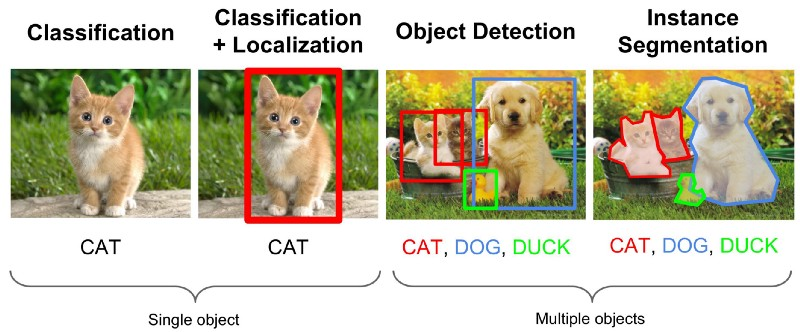
\includegraphics[width=\textwidth]{grafika/problemy.jpeg}
    \caption{Różne problemy dla obrazków}
    \label{fig_problemy}
\end{figure}
\end{frame}

\begin{frame}{Po co nam wykrywanie obiektów?}
\begin{itemize}
    \item Autonomiczne samochody
    \item Wykrywanie twarzy (Facebook, aparaty)
    \item Śledzenie obiektów (automatyczny ruch kamery np. za piłką)
    \item Liczenie ludzi (badanie ruchu w sklepach, demonstracje, festiwale)
    \item Podobnie liczenie innych obiektów, np. samochodów
    \item \href{https://tryolabs.com/blog/2017/08/30/object-detection-an-overview-in-the-age-of-deep-learning/}{Visual Search Engine}
\end{itemize}

\begin{block}{Na zachętę}
    \href{https://www.youtube.com/watch?v=VOC3huqHrss&t}{Filmik promujący YOLO}
\end{block}
\end{frame}

\begin{frame}{Zbiory danych}

\begin{itemize}
    \item \href{http://host.robots.ox.ac.uk/pascal/VOC/voc2011/examples/index.html}{PASCAL} Visual Object Classification (10 000 obrazków, 20 klas, porządne bounding boxy)
    \item \href{https://www.kaggle.com/c/imagenet-object-detection-challenge}{ImageNet} (500 000 obrazków, 200 klas, z bounding boxami)
    \item \href{http://cocodataset.org/\#explore}{Common Objects in COntext} (120 000 obrazków, 80 kategorii)
\end{itemize}
\end{frame}

\begin{frame}{Sposoby oceniania detektorów}

\begin{itemize}
    \item Intersection over Union (IoU)
    \item Precision ($\frac{TP}{TP+FP}$) i recall ($\frac{TP}{TP+FN}$)
    \item TP: dobra klasa, IoU $ > t$
    \item Average Precision 
    \begin{align*}
        AP &= \frac{1}{11} \sum_{r \in \{0.0, \ldots, 1.0\}} max_{r' \geq r} p(r') \\ p(r) &- \text{maksymalna precyzja dla zadanego recall}
    \end{align*} 
    \item mean Average Precision (mAP) - średnia z AP po wszystkich klasach
\end{itemize}
\end{frame}

\begin{frame}{Wczesne metody - okno przesuwne + klasyfikacja}
\begin{figure}
    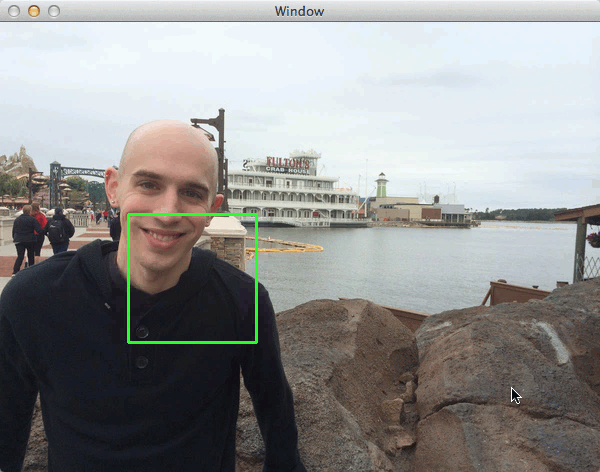
\includegraphics[height=0.5\textheight]{grafika/sliding.png}
\end{figure}
\begin{alertblock}{Problemy}
\begin{itemize}
    \item Wielkość okna, obiektów
    \item Skumulowanie wyników
    \item Bardzo dużo razy uruchamiany klasyfikator
\end{itemize}
\end{alertblock}
\end{frame}

\begin{frame}{Pierwsze podejście - OverFeat (2013)}
    \begin{itemize}
        \item Okno przesuwne = sploty
        \item Sieć konwolucyjna do wyciągniecia feature map
        \item Multiscale classicication (dużo rozmiarów i uśrednienie wyników)
        \begin{figure}[H]
        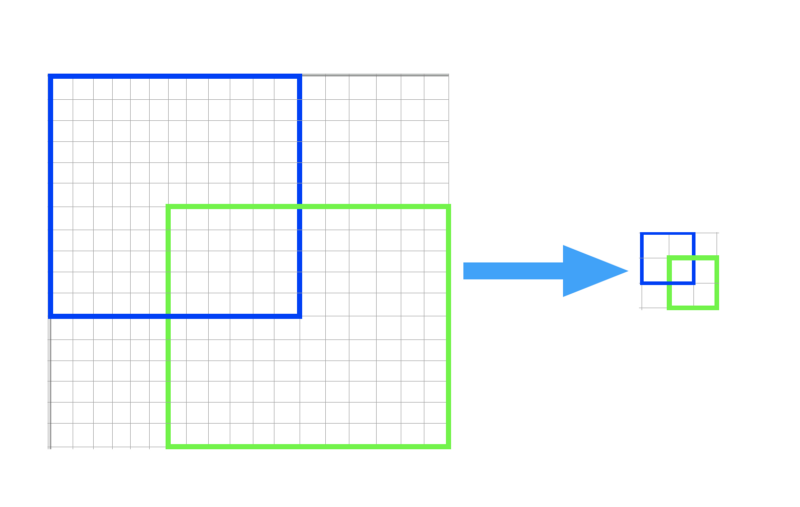
\includegraphics[height=0.3\textheight]{grafika/multiscale.png}
        \end{figure}
        \item Do detekcji - dodatkowa klasa tło
        \item Do lokalizacji - dodatkowe warstwy aplikowane na FM wyznaczające współrzędne i rozmiary (jednego obiektu)
        \item Łączenie boxów - uśrednianie współrzędnych
    \end{itemize}
\end{frame}


\begin{frame}{Region-based Convolutional Network (R-CNN, 2014)}
Motywacja: propozycje regionów
\begin{figure}
    \centering
    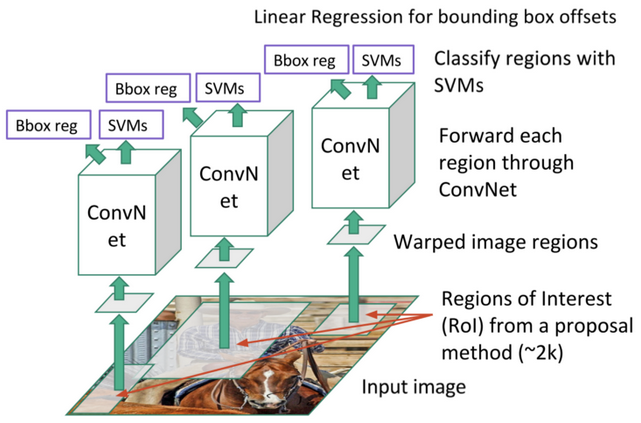
\includegraphics[width=\textwidth]{grafika/rcnn.png}
    \caption{Schemat R-CNN}
    \label{fig_rcnn1}
\end{figure}
\end{frame}

\begin{frame}{R-CNN}
\begin{itemize}
    \item Selective Search - preprocessing + grupowanie hierarchiczne \\
    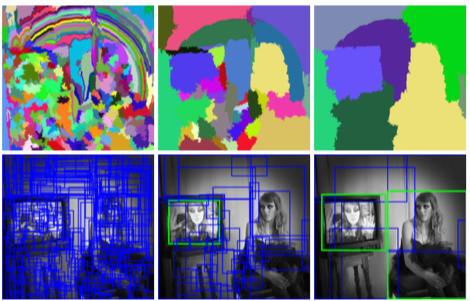
\includegraphics[height=0.5\textheight]{grafika/selective.png}
    \item Niezależnie trenowana sieć konwolucyjna do wyciągania feature map
    \item Małe FM $\Rightarrow$ szybka klasyfikacja za pomocą SVM
    \item Regresja liniowa dla BB
\end{itemize}

\end{frame}

\begin{frame}{Fast R-CNN (2015)} 
Motywacja: przyspieszenie R-CNN \\
Rozwiązanie: jedno przejście przez sieć konwolucyjną
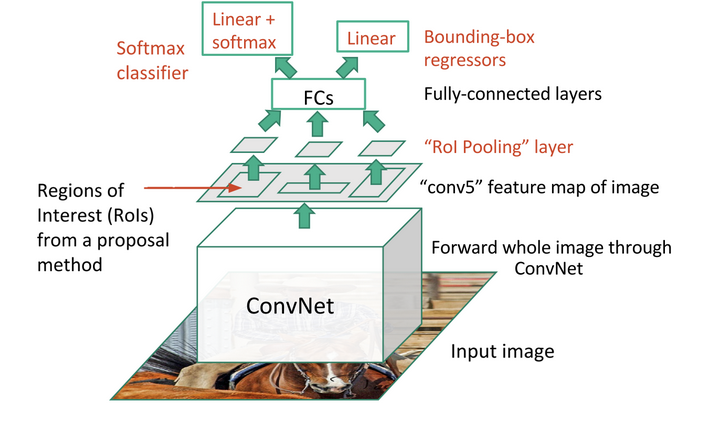
\includegraphics[width=\textwidth]{grafika/fastrcnn.png}
\end{frame}

\begin{frame}{Fast R-CNN}
\begin{itemize}
    \item Propozycje regionów z feature mapy 
    \item Każdy propozycja jest wrzucana do FC oddzielnie
    \item Roi Pooling - feature mapy regionów do stałego rozmiaru 
\end{itemize}
\end{frame}

\begin{frame}{Faster R-CNN (2016)}
Motywacja: wyrzućmy wąskie gardło - Selective Search
\begin{figure}
    \centering
    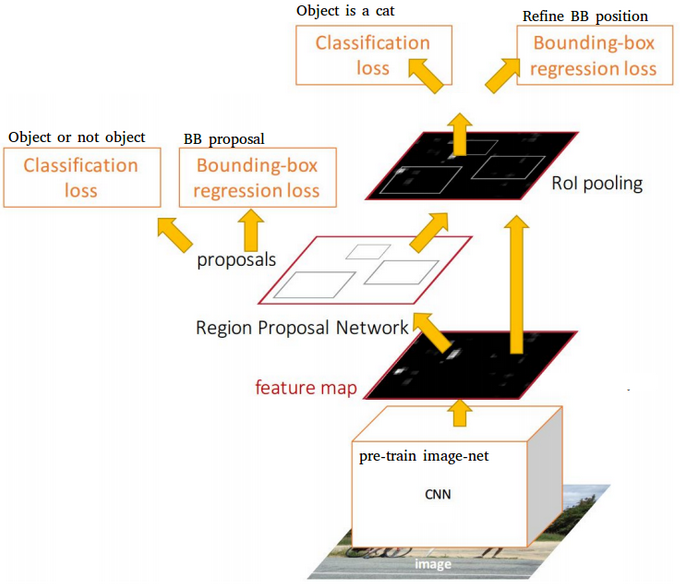
\includegraphics[height=0.75\textheight]{grafika/fasterrcnn.png}
\end{figure}
\end{frame}

\begin{frame}{Faster R-CNN}

\begin{itemize}
    \item RPN - max k regionów ze współrzędnymi i scorem
    \item Przesuwne okno do warstwy FC (ale dzieje się równocześnie)
    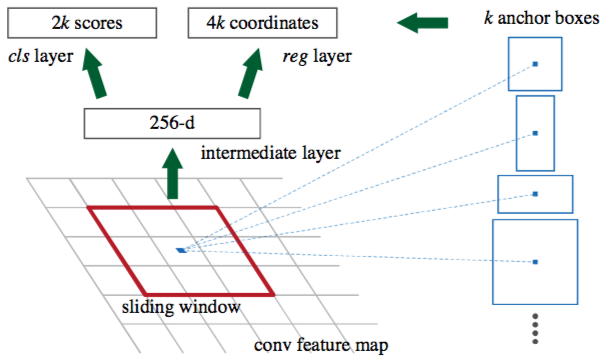
\includegraphics[height=0.6\textheight]{grafika/rpn.png}
    \item RPN + CNN (mechanizm uwagi)
\end{itemize}
    
\end{frame}


\begin{frame}{YOLO (2016)}
\begin{itemize}
    \item Bounding boxes i klasyfikacja naraz - jedno przejście przez sieć
    \item Globalna analiza obrazka
\end{itemize}
\begin{figure}
    \centering
    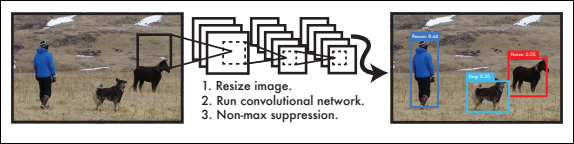
\includegraphics[width=\textwidth]{grafika/yolo-schemat.png}
    \caption{Schemat działania YOLO}
    \label{fig_yolo_schemat}
\end{figure}
\end{frame}


\begin{frame}{Bardziej szczegółowo}
    \begin{itemize}
        \item Siatka $S\times S$
        \item Jedna komórka $\Rightarrow$ jeden obiekt
        \item $B$ bounding boxów w każdej komórce
        \item Box: (x,y,w,h,score)
        \item Przykład PASCAL VOC: $B=2, C=20, S=7 \Rightarrow$  tensor $7 \times 7 \times 30$ 
    \end{itemize}
\end{frame}

\begin{frame}{Bounding boxes}
\begin{figure}
    \centering
    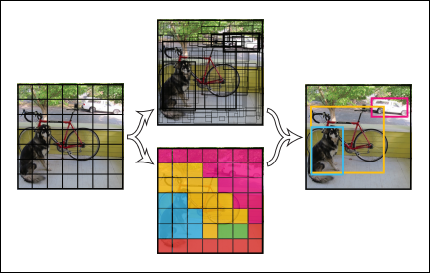
\includegraphics[width=\textwidth]{grafika/yolo-boxy.png}
    \caption{Bounding boxes}
    \label{fig_boxes}
\end{figure}
\end{frame}

\begin{frame}{Łączenie BB - non-maximal suppression}
\begin{itemize}
    \item Sortujemy boxy po scorach
    \item Ignoruj box, jeśli jakiś poprzedni ma IoU $\geq 0.5$ z aktualnym boxem (i oczywiście ta sama klasa)
    \item Przetwórz tak wszytskie
\end{itemize}
    
\end{frame}


\begin{frame}{Architektura sieci}
\begin{figure}
    \centering
    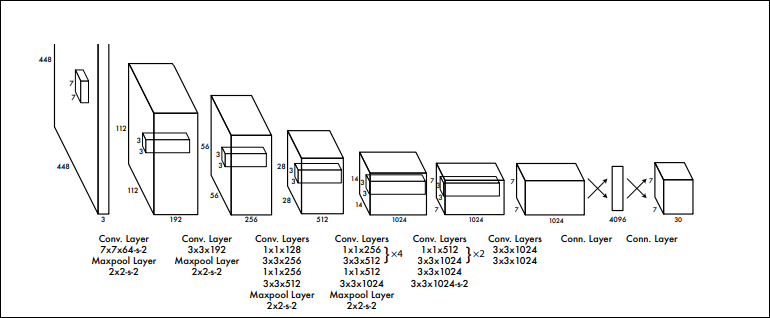
\includegraphics[width=\textwidth]{grafika/yolo-architektura.png}
    \caption{Architektura sieci}
    \label{fig_architektura}
\end{figure}
\end{frame}

\begin{frame}{Kara}
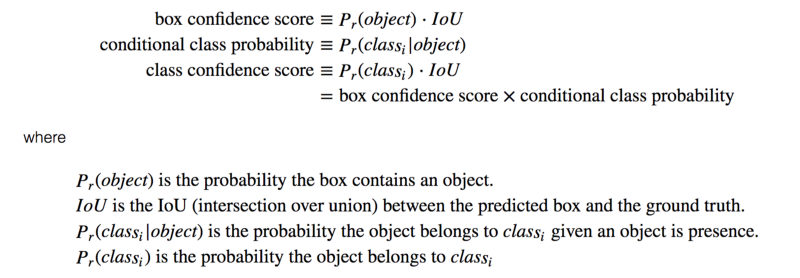
\includegraphics[width=\textwidth]{grafika/confidence.png} \\
W karze uwzględniamy:
\begin{itemize}
    \item kara za klasyfikację
    \item kara za lokalizację
    \item kara za score boxów
\end{itemize}
\end{frame}


\begin{frame}{YOLO - generalizacja}
\begin{figure}
    \centering
    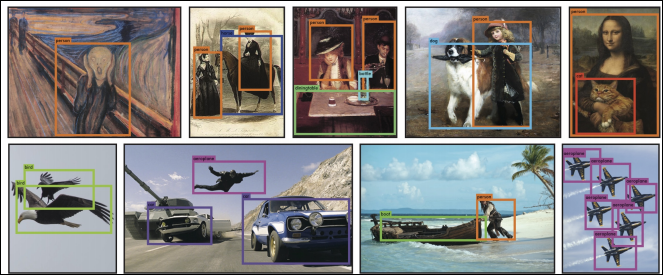
\includegraphics[width=0.9\textwidth]{grafika/yolo-natural.png}

\end{figure}
\uncover<2->{
\begin{alertblock}{Problemy}
\begin{itemize}
    \item Małe obiekty blisko siebie
    \item Mniejszy mAP niż dla innych metod
\end{itemize}
\end{alertblock}
}
\end{frame}

\begin{frame}{YOLOv2 (2016)}
\begin{itemize}
    \item Batch normalization, zwiększenie rozdzielczości
    \item Ustalone rozmiary boxów na początku - standardowe kształty
    \item Anchor boxy wyznaczane k-means z dystansem bazującym na IoU
    \begin{figure}[H]
        \centering
        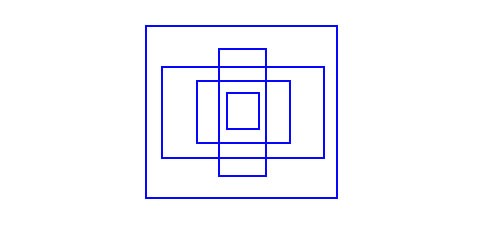
\includegraphics[height=0.15\textheight]{grafika/boxy.jpeg}
    \end{figure}
    \item Przeniesienie prawdopodobieństw klas do boxów: tensor $(S,S, B\times(5+C)) $, $B=5, S=13$
    \item Fine grained features - wykrywanie mniejszych obiektów za pomocą FM w większej rozdzielczości
    \item MultiScale Training - co 10 batchów zmieniają rozdzielczości obrazka (można bo same warswy splotowe)
    \item Zmiana sieci wcześniej trenowanej sieci splotowej
\end{itemize}
\end{frame}

\begin{frame}[allowframebreaks]{YOLO9000}
\begin{itemize}
    \item Połączenie zbiorów danych detekcji i klasyfikacji
    \item Detekcję i klasyfikację trenujemy oddzielnie
    \item Problemy: łączenie nazw klas, rozłączne klasy bo softmax
    \begin{figure}
        \centering
        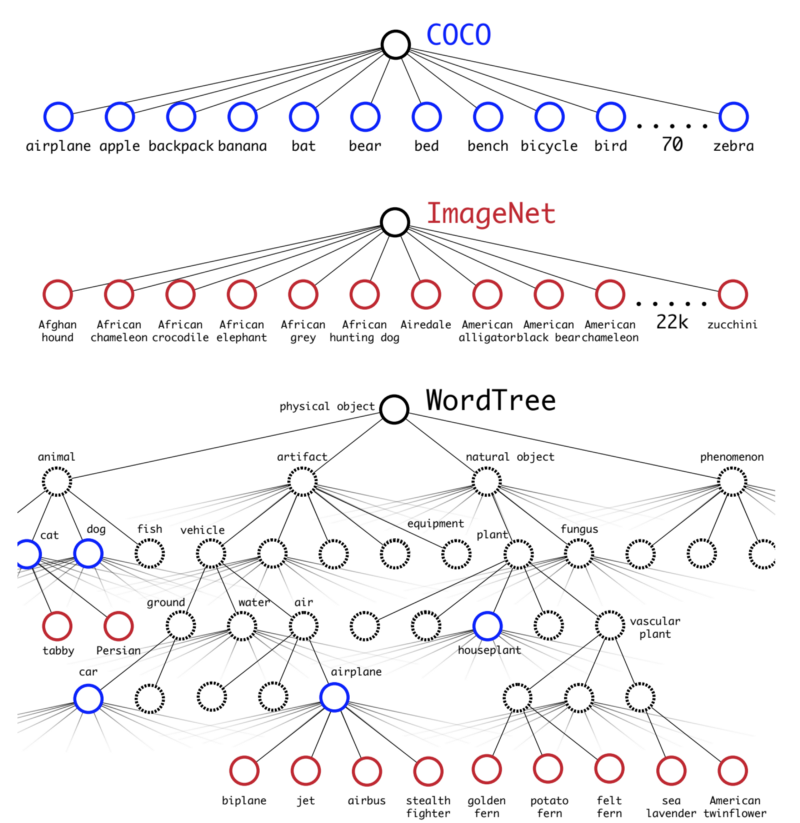
\includegraphics[height=0.6\textheight]{grafika/wordtree.png}
    \end{figure}
    \item Błędy klasyfikacji zarówno dla liścia jak i przodków - wyciąga wspólne cechy
    \item Trenowane na COCO + 9000 klas z ImageNet
    \item Testowane na ImageNet do detekcji (tylko $44/200$ wspólnych klas z COCO)
\end{itemize}
    
\end{frame}

\begin{frame}{Inne metody}
\begin{itemize}
    \item Single Shot Detector (2016)
    \item Neural Architecture Search Net (NASNet, 2017)
    \item Mask Region-based Convolutional Network (Mask R-CNN, 2017) - również segmentacja obrazka
    \item RetinaNet (2018)
\end{itemize}
\end{frame}

\begin{frame}{Porównanie działania różnych metod detekcji}
\begin{figure}
    \centering
    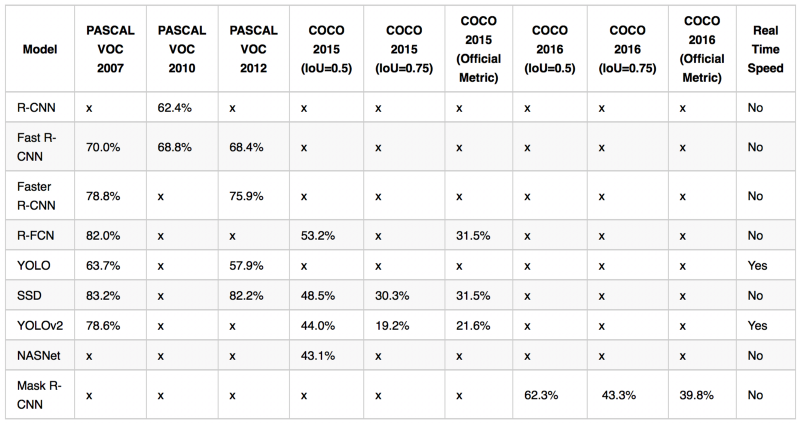
\includegraphics[width=\textwidth]{grafika/porownanie.png}
    \caption{Porównanie mAP}
    \label{fig_comp}
\end{figure}
\end{frame}

\begin{frame}{YOLOv3 (2018)}
\begin{itemize}
    \item Zwiększenie $S,B$, zmiana sieci splotowej
    \item Zmiana kary za BB, wiele klas do jednego obiektu
    \item Feature Pyramid Network (FPN)
    \begin{figure}
        \centering
        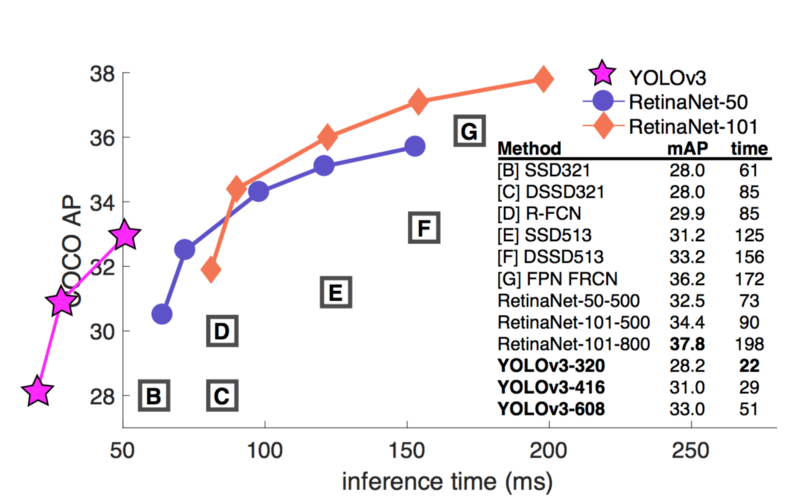
\includegraphics[height=0.65\textheight]{grafika/yolov3.png}
    \end{figure}
\end{itemize}
    
\end{frame}

    
\begin{frame}[allowframebreaks]{Bibliografia} 

\nocite{*}
\footnotesize{
\bibliography{biblio1}
\bibliographystyle{plain}
}
\end{frame}

\appendix
\backupbegin

\backupend
\end{document}
